\documentclass[t, aspectratio=169, 10pt]{beamer}
\usepackage{elmagTemplate}

% Utility packages
\newcommand\SLASH{\char`\\} % Used for command examples
\usepackage{array} % Array and tabular enhancements
\newcolumntype{C}[1]{>{\centering\arraybackslash}p{#1}} % Centered column type
\usepackage{amsmath, amssymb, amsfonts, physics, tabu, pgfplots}
\usepackage{tikz-3dplot}

\usepackage[school,simplified]{pgf-umlcd}
\usetikzlibrary{calc}
\usetikzlibrary{positioning}
\usetikzlibrary{shapes.geometric, arrows}
\usepackage{matlab-prettifier}
\usepackage{mathtools}

\tikzstyle{startstop} = [rectangle, rounded corners, 
minimum width=3cm, 
minimum height=1cm,
text centered, 
draw=black, 
fill=red!30]

\tikzstyle{io} = [trapezium, 
trapezium stretches=true, % A later addition
trapezium left angle=70, 
trapezium right angle=110, 
minimum width=3cm,
minimum height=1cm, text centered,
align = center,
draw=black, fill=blue!30]

\tikzstyle{process} = [rectangle, 
minimum width=3cm, 
minimum height=1cm, 
text centered, 
draw=black,
align=center,
fill=orange!30]


\tikzstyle{decision} = [diamond, 
minimum width=2cm, 
minimum height=1cm, 
text centered,
align=center,
draw=black, 
fill=green!30]
\tikzstyle{arrow} = [thick,->,>=stealth]

% Metadata
\title[\textsc{Matlab} competition task]{Vigen\`ere cipher cracker}
\author[Tom\'a\v{s} Mach\'a\v{c}ek]{Tom\'a\v{s} Mach\'a\v{c}ek}
\date[\today]{\today}

% Begin Document
\begin{document}

% Title Slide
\begin{frame}
    \titlepage
\end{frame}

\section{Code structure}
\begin{frame}{Class program structure}
    \begin{figure}[h!]
        \centering
        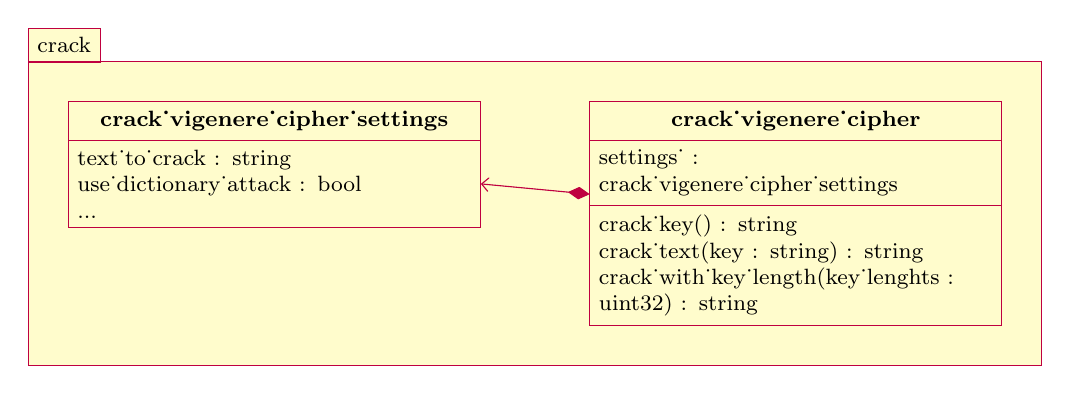
\begin{tikzpicture}[font=\footnotesize] % reduce fontsize
            \begin{package}{crack}
            \begin{class}[text width = 5cm]{\detokenize{crack_vigenere_cipher_settings}}{0,0}
                \attribute{\detokenize{text_to_crack} : string}
                \attribute{\detokenize{use_dictionary_attack} : bool}
                \attribute{...}
            \end{class}
                \begin{class}[text width = 5cm, xshift = 4cm]{\detokenize{crack_vigenere_cipher}}{\detokenize{crack_vigenere_cipher_settings}.north east}
                    \attribute{\detokenize{settings_} : \detokenize{crack_vigenere_cipher_settings}}
                    \operation{\detokenize{crack_key()} : string}
                    \operation{\detokenize{crack_text(key : string)} : string}
                    \operation{\detokenize{crack_with_key_length(key_lenghts : uint32)} : string}
                \end{class}
            \end{package}
            \composition{\detokenize{crack_vigenere_cipher}}{}{}{\detokenize{crack_vigenere_cipher_settings}}
        \end{tikzpicture}
        \caption{Basic code structure class-vice}
    \end{figure}
\end{frame}

\begin{frame}{crackVigenereCipher function}
    \vspace{2em}
    \lstinputlisting[frame=single,numbers=left,style=Matlab-Pyglike]{../src/crackVigenereCipher.m}
\end{frame}

\begin{frame}{crack.crack\_key() flowchart}
    \begin{figure}[h!]
        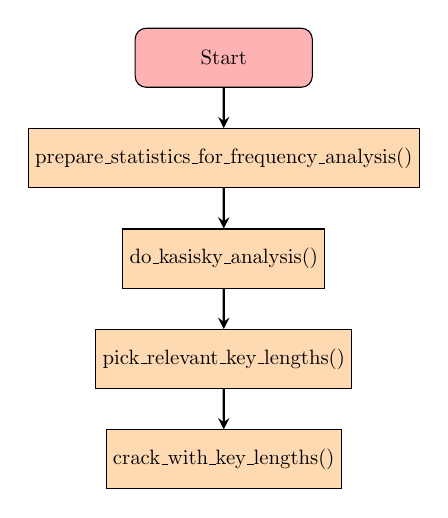
\begin{tikzpicture}[node distance=1.7cm, scale=0.75, every node/.style={transform shape}]
            \node (start) [startstop] {Start};
            \node (pro1) [process, below of=start] {prepare\_statistics\_for\_frequency\_analysis()};
            \node (pro2) [process, below of=pro1] {do\_kasisky\_analysis()};
            \node (pro3) [process, below of=pro2] {pick\_relevant\_key\_lengths()};
            \node (pro4) [process, below of=pro3] {crack\_with\_key\_lengths()};

            \draw [arrow] (start) -- (pro1);
            \draw [arrow] (pro1) -- (pro2);
            \draw [arrow] (pro2) -- (pro3);
            \draw [arrow] (pro3) -- (pro4);
        \end{tikzpicture}
    \end{figure}
\end{frame}

\begin{frame}{crack.crack\_with\_key\_length() flowchart}
    \begin{figure}[h!]
        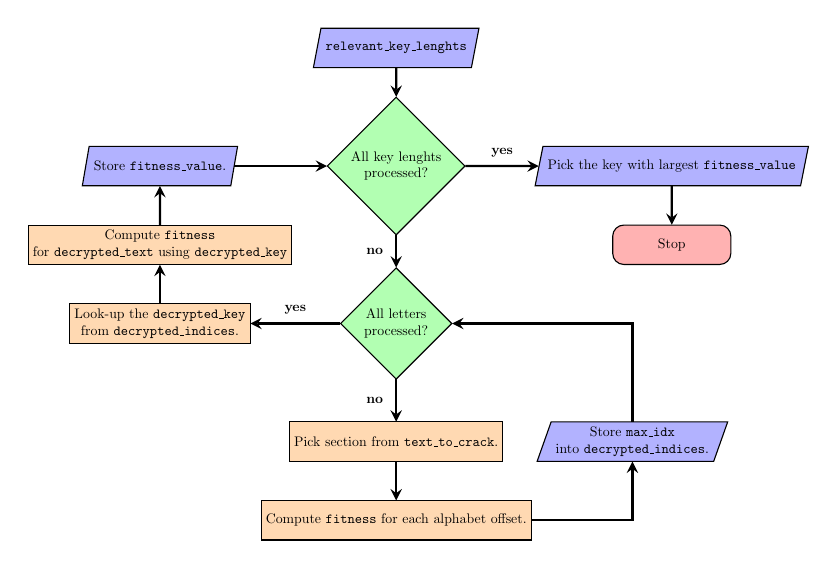
\begin{tikzpicture}[node distance=2cm, scale=0.5, every node/.style={transform shape}]
            \node (in1) [io] {\texttt{relevant\_key\_lenghts}};
            \node (dec1) [decision, below of=in1, yshift=-1cm] {All key lenghts\\ processed?};
            \node (dec2) [decision, below of=dec1, yshift=-2cm] {All letters\\ processed?};
            \node (pro1) [process, below of=dec2, yshift=-1cm] {Pick section from \texttt{text\_to\_crack}.};
            \node (pro2) [process, below of=pro1] {Compute \texttt{fitness} for each alphabet offset.};
            \node (out1) [io, right of=pro1, xshift=4cm] {Store \texttt{max\_idx}\\ into \texttt{decrypted\_indices}.};
            \node (pro3) [process, left of=dec2, xshift=-4cm] {Look-up the \texttt{decrypted\_key}\\ from \texttt{decrypted\_indices}.};
            \node (pro4) [process, above of=pro3] {Compute \texttt{fitness}\\ for \texttt{decrypted\_text} using \texttt{decrypted\_key}};
            \node (out2) [io, above of=pro4] {Store \texttt{fitness\_value}.};
            \node (out3) [io, right of=dec1, xshift=5cm] {Pick the key with largest \texttt{fitness\_value}};
            \node (stop) [startstop, below of=out3] {Stop};

            \draw [arrow] (in1.south) -- (dec1);
            \draw [arrow] (dec1) -- node[anchor=south, left=0.2cm] {\textbf{no}} (dec2);
            \draw [arrow] (dec2) -- node[anchor=south, left=0.2cm] {\textbf{no}} (pro1);
            \draw [arrow] (pro1) -- (pro2);
            \draw [arrow] (pro2) -| (out1);
            \draw [arrow] (out1) |- (dec2);
            \draw [arrow] (dec2) -- node[anchor=west, above=0.1cm] {\textbf{yes}} (pro3);
            \draw [arrow] (pro3) -- (pro4);
            \draw [arrow] (pro4) -- (out2);
            \draw [arrow] (out2) -- (dec1);
            \draw [arrow] (dec1) -- node[anchor=east, above=0.1cm] {\textbf{yes}} (out3);
            \draw [arrow] (out3) -- (stop);
        \end{tikzpicture}
    \end{figure}
\end{frame}

\begin{frame}{Fitness computation}
    \begin{itemize}
        \item Suppose two sequences $A = (a_n)_{n = 1}^{N}$ and $B = (b_n)_{n = 1}^{N}$, $a_n, b_n \in \mathbb{N}$. Then we define a fitenss operator
        \begin{equation*}
            \mathcal{F}(A, B) \coloneqq \frac{\braket{A}{B}_{\ell^2}}{\|A\|_{\ell^2} \|B\|_{\ell^2}} = \frac{\sum_{n = 1}^{N} a_nb_n}{\sqrt{\sum_{n = 1}^{N}a_n^2} \sqrt{\sum_{n = 1}^{N}b_n^2}}.
        \end{equation*}
    \end{itemize}
\end{frame}

\section*{Questions}
\begin{frame}
    \centering
    \vspace{2cm}
    {\Huge \textcolor{elmagBlueL}{Questions?}}
\end{frame}


\end{document}

